% filename: ProgramPlotsA.tex
\documentclass[11pt]{article}
\include{PhysNote}
\usepackage{srcltx}

\usepackage{ifpdf} % to switch between .eps and .png file types for images (for compiling)

\title{Program Plots A}
\author{Andrew Forrester}


\begin{document}
\maketitle
\tableofcontents


%\newpage
\section{Files}

\begin{comment}
plot_a0atTcVsPressure.png
plot_RotonEnergyAtTcVsPressure.png
plot_RotonEnergyVsTemp_atTc.png
\end{comment}

\squishlist
  \item \verb|plot_a0atTcVsPressure.png|
  \item \verb|plot_RotonEnergyAtTcVsPressure.png|
  \item \verb|plot_RotonEnergyVsTemp_atTc.png|
\squishend



\section{Smallest Vortex Diameters}


\begin{center}
\begin{tabular}[\textwidth]{p{8.5cm}p{8.5cm}}
\ifpdf
  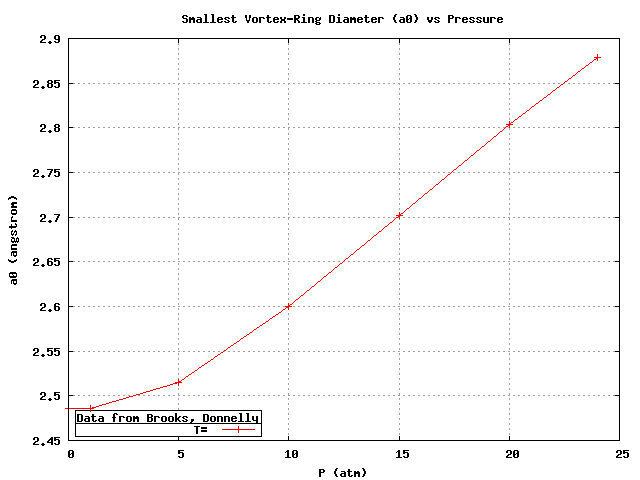
\includegraphics[width=8.5cm]{plot_a0atTcVsPressure.png}\newline
  \verb|plot_a0atTcVsPressure.png|
\else
  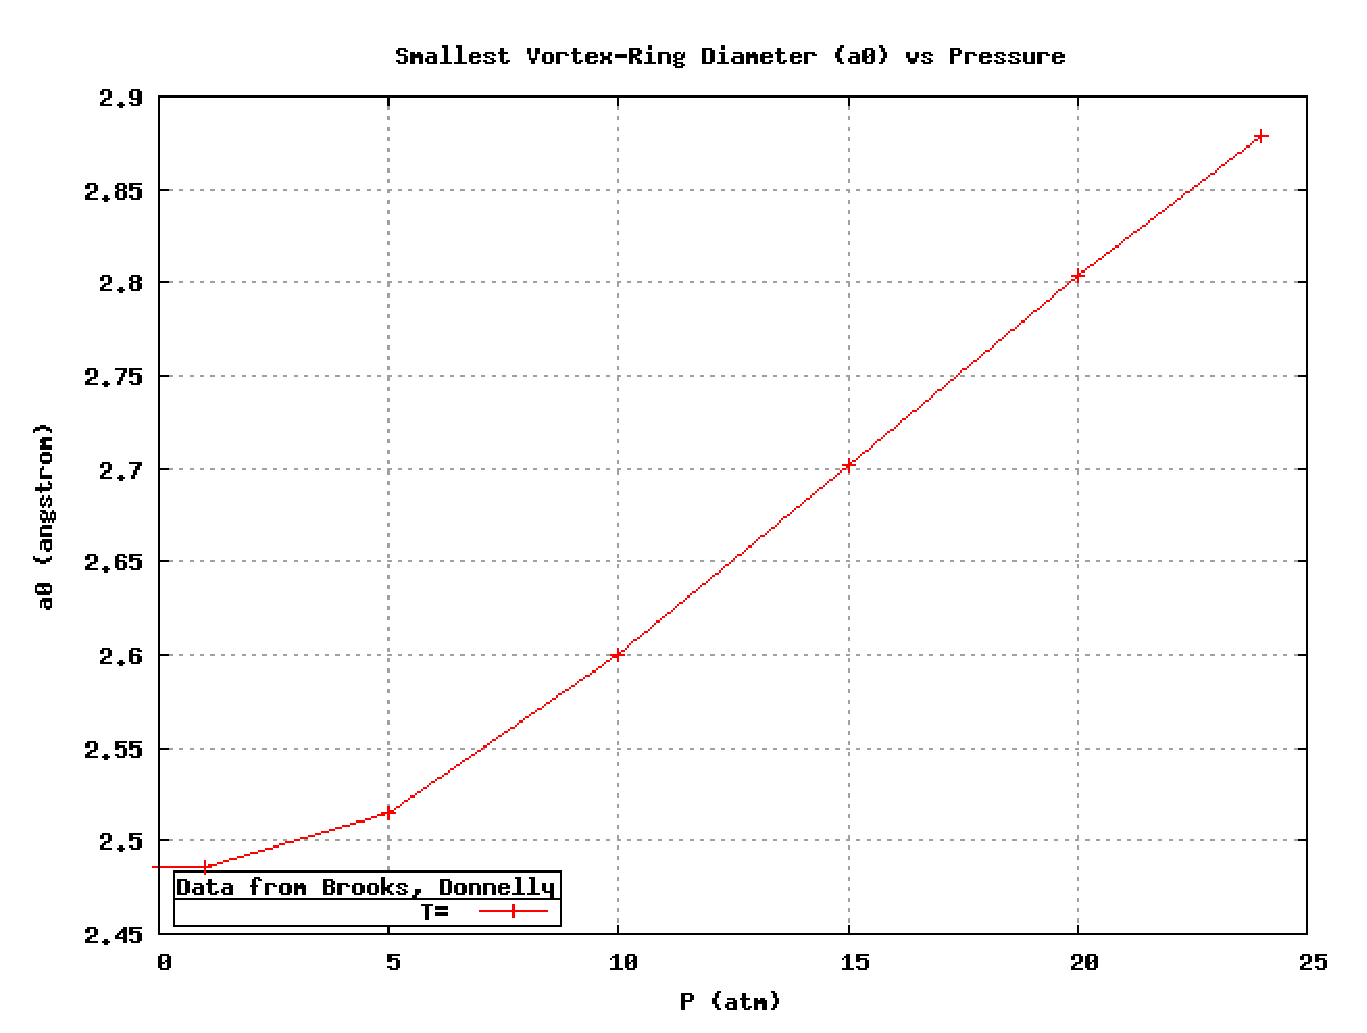
\includegraphics[width=8.5cm]{plot_a0atTcVsPressure.eps}\newline
  \verb|plot_a0atTcVsPressure.eps|
\fi
&
 \\
\end{tabular}
\end{center}


\newpage
\section{Roton Energy Gap Data and Calculations}

\begin{center}
\begin{tabular}[\textwidth]{p{8.5cm}p{8.5cm}}
\ifpdf
  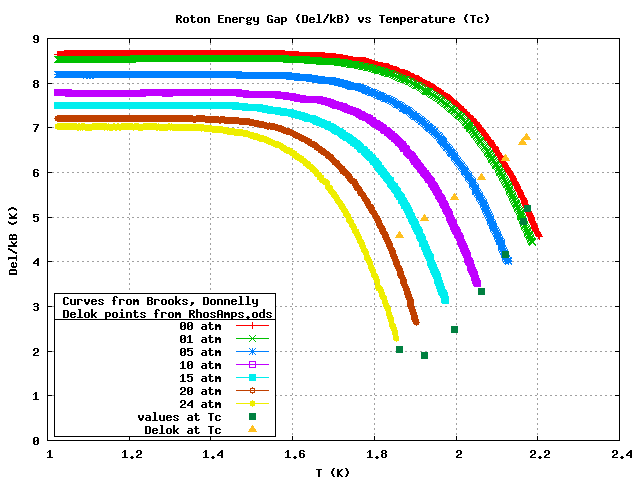
\includegraphics[width=8.5cm]{plot_RotonEnergyVsTemp_atTc.png}\newline
  \verb|plot_RotonEnergyVsTemp_atTc.png|
\else
  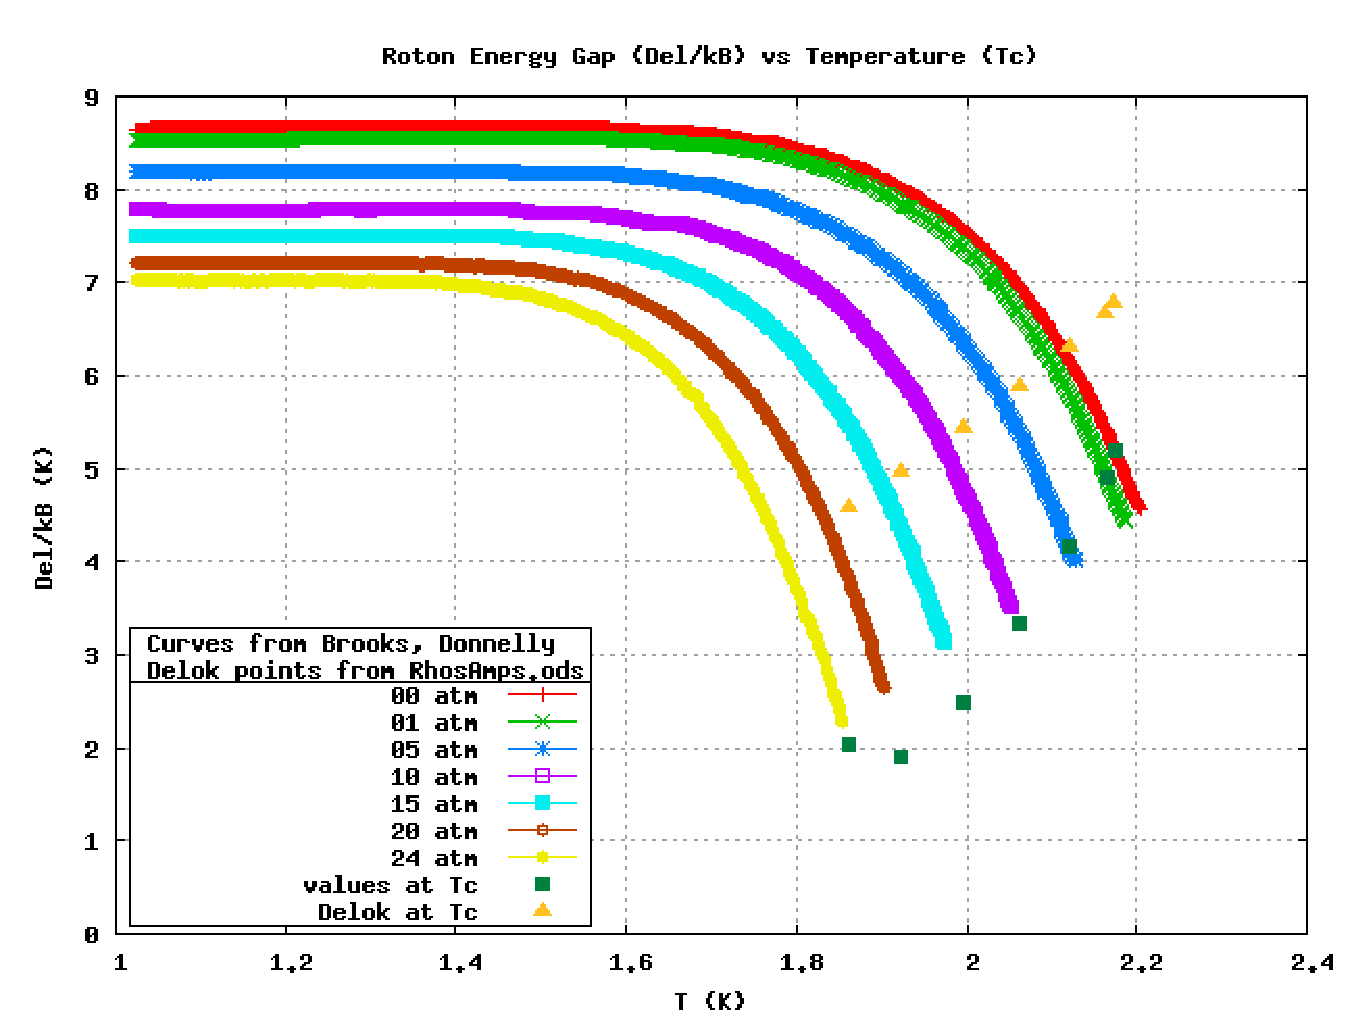
\includegraphics[width=8.5cm]{plot_RotonEnergyVsTemp_atTc.eps}\newline
  \verb|plot_RotonEnergyVsTemp_atTc.eps|
\fi
&
\ifpdf
  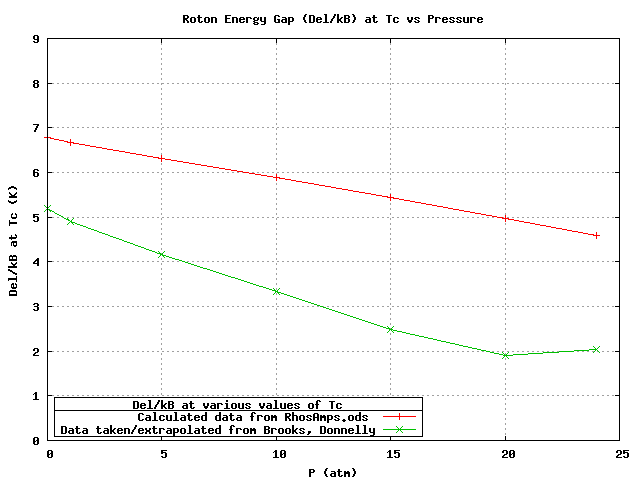
\includegraphics[width=8.5cm]{plot_RotonEnergyAtTcVsPressure.png}\newline
  \verb|plot_RotonEnergyAtTcVsPressure.png|
\else
  \includegraphics*[width=8.5cm]{plot_RotonEnergyAtTcVsPressure.eps}\newline
  \verb|plot_RotonEnergyAtTcVsPressure.eps|
\fi
 \\
\end{tabular}
\end{center}


\end{document}